\documentclass[tikz,border=8pt]{standalone}
\usepackage[utf8]{inputenc}
\usetikzlibrary{arrows.meta,fit,backgrounds,shadows}

% module names: smaller monospace so the longest ones fit in a block
\newcommand{\modname}[1]{{\scriptsize\ttfamily #1}}

% Etapa 1 (commit 91c57c9): loopback 10GBASE-R en los cuatro carriles del
% QSFP28. Cada trama que llega del PC por un carril se devuelve por el mismo
% carril a través de una FIFO asíncrona, sin pila IP.

\begin{document}
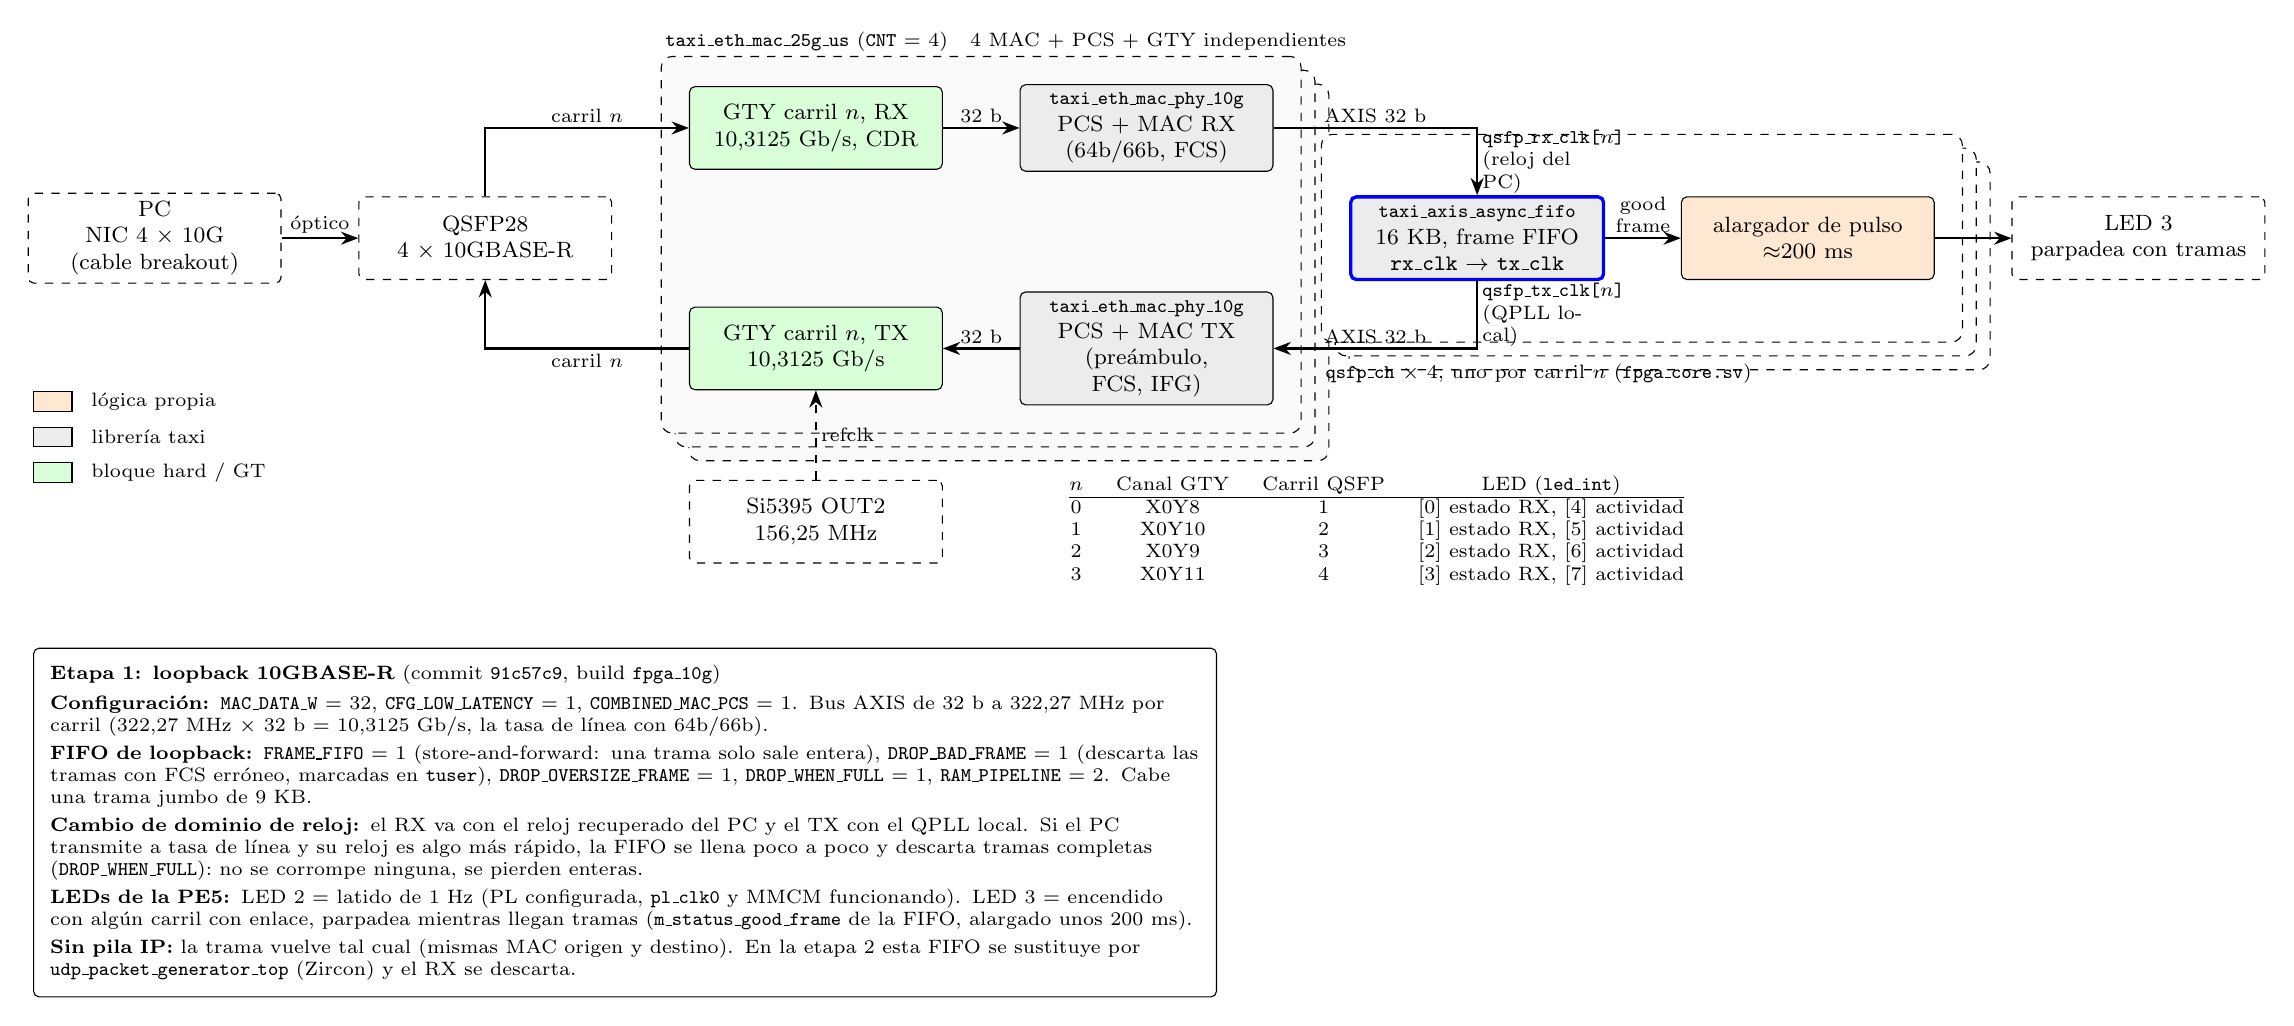
\begin{tikzpicture}[
    x=1.235cm,
    font=\footnotesize,
    >={Stealth[length=2.2mm]},
    blk/.style={draw, rounded corners=2pt, minimum height=1.05cm,
                text width=3.0cm, align=center, inner sep=3pt},
    gen/.style={blk, fill=orange!18},
    taxi/.style={blk, fill=gray!15},
    soft/.style={blk, fill=gray!15},
    hard/.style={blk, fill=green!15},
    ext/.style={blk, fill=white, dashed},
    grp/.style={draw, dashed, rounded corners=4pt},
    lbl/.style={font=\scriptsize, inner sep=1.5pt},
    flow/.style={->, thick},
]

% ---------------------------------------------------------------- external
\node[ext]  (pc)      at (-3.4,-1.4) {PC\\NIC 4 $\times$ 10G\\(cable breakout)};
\node[ext]  (qsfp)    at (0,-1.4)    {QSFP28\\4 $\times$ 10GBASE-R};
\node[ext]  (si5395)  at (3.4,-5.0)  {Si5395 OUT2\\156,25 MHz};

% ---------------------------------------------------------------- RX row
\node[hard] (gtyrx)   at (3.4,0)     {GTY carril $n$, RX\\10,3125 Gb/s, CDR};
\node[soft] (macrx)   at (6.8,0)     {\modname{taxi\_eth\_mac\_phy\_10g}\\PCS + MAC RX\\(64b/66b, FCS)};

% ---------------------------------------------------------------- TX row
\node[hard] (gtytx)   at (3.4,-2.8)  {GTY carril $n$, TX\\10,3125 Gb/s};
\node[soft] (mactx)   at (6.8,-2.8)  {\modname{taxi\_eth\_mac\_phy\_10g}\\PCS + MAC TX\\(preámbulo, FCS, IFG)};

% ---------------------------------------------------------------- loopback FIFO
\node[taxi, draw=blue, very thick]
            (fifo)    at (10.2,-1.4) {\modname{taxi\_axis\_async\_fifo}\\16 KB, frame FIFO\\\texttt{rx\_clk} $\to$ \texttt{tx\_clk}};
\node[gen]  (act)     at (13.6,-1.4) {alargador de pulso\\$\approx$200 ms};
\node[ext]  (led)     at (17,-1.4)   {LED 3\\parpadea con tramas};

% ---------------------------------------------------------------- arrows
\draw[flow] (pc)      -- node[lbl, above] {óptico} (qsfp);
\draw[flow] (qsfp.north) |- node[lbl, above, pos=0.75] {carril $n$} (gtyrx.west);
\draw[flow] (gtyrx)   -- node[lbl, above] {32 b} (macrx);
\draw[flow] (macrx.east) -| node[lbl, above, pos=0.25] {AXIS 32 b} node[lbl, right, pos=0.75, text width=1.6cm] {\texttt{qsfp\_rx\_clk[$n$]}\\(reloj del PC)} (fifo.north);
\draw[flow] (fifo.south) |- node[lbl, right, pos=0.25, text width=1.6cm] {\texttt{qsfp\_tx\_clk[$n$]}\\(QPLL local)} node[lbl, above, pos=0.75] {AXIS 32 b} (mactx.east);
\draw[flow] (mactx)   -- node[lbl, above] {32 b} (gtytx);
\draw[flow] (gtytx.west) -| node[lbl, below, pos=0.25] {carril $n$} (qsfp.south);
\draw[flow] (fifo)    -- node[lbl, above, text width=1.4cm, align=center] {good\\frame} (act);
\draw[flow] (act)     -- (led);
\draw[flow, dashed] (si5395) -- node[lbl, right] {refclk} (gtytx);

% ---------------------------------------------------------------- groups
\begin{scope}[on background layer]
    \node[grp, fit=(gtyrx)(macrx)(gtytx)(mactx), inner sep=10pt, fill=gray!4,
          double copy shadow={shadow xshift=5pt, shadow yshift=-5pt}] (macgrp) {};
    \node[grp, fit=(fifo)(act), inner xsep=10pt, inner ysep=22pt, fill=white,
          double copy shadow={shadow xshift=5pt, shadow yshift=-5pt}] (chgrp) {};
\end{scope}
\node[lbl, anchor=south west, align=left] at (macgrp.north west)
    {\texttt{taxi\_eth\_mac\_25g\_us} (\texttt{CNT} = 4)\quad 4 MAC + PCS + GTY independientes};
\node[lbl, anchor=north west, align=left] at ([yshift=-6pt]chgrp.south west)
    {\texttt{qsfp\_ch} $\times$ 4, uno por carril $n$ (\texttt{fpga\_core.sv})};

% ---------------------------------------------------------------- legend
\begin{scope}[shift={(-4.65,-3.6)}, every node/.style={font=\scriptsize, anchor=west}]
    \draw[fill=orange!18] (0,0)     rectangle +(0.4,0.25); \node at (0.5,0.125)  {lógica propia};
    \draw[fill=gray!15]   (0,-0.45) rectangle +(0.4,0.25); \node at (0.5,-0.325) {librería taxi};
    \draw[fill=green!15]  (0,-0.9)  rectangle +(0.4,0.25); \node at (0.5,-0.775) {bloque hard / GT};
\end{scope}

% ---------------------------------------------------------------- lane table
\node[anchor=north west, font=\scriptsize, inner sep=0pt] at (6.0,-4.4) {%
    \begin{tabular}{@{}cccc@{}}
        $n$ & Canal GTY & Carril QSFP & LED (\texttt{led\_int})\\\hline
        0 & X0Y8  & 1 & [0] estado RX, [4] actividad\\
        1 & X0Y10 & 2 & [1] estado RX, [5] actividad\\
        2 & X0Y9  & 3 & [2] estado RX, [6] actividad\\
        3 & X0Y11 & 4 & [3] estado RX, [7] actividad\\
    \end{tabular}};

% ---------------------------------------------------------------- notes
\node[draw, rounded corners=2pt, anchor=north west, text width=14.6cm, align=left,
      font=\scriptsize, inner sep=6pt] at (-4.65,-6.6) {%
    \textbf{Etapa 1: loopback 10GBASE-R} (commit \texttt{91c57c9}, build \texttt{fpga\_10g})\\[3pt]
    \textbf{Configuración:} \texttt{MAC\_DATA\_W} = 32, \texttt{CFG\_LOW\_LATENCY} = 1,
    \texttt{COMBINED\_MAC\_PCS} = 1. Bus AXIS de 32 b a 322,27 MHz por carril
    (322,27 MHz $\times$ 32 b = 10,3125 Gb/s, la tasa de línea con 64b/66b).\\[2pt]
    \textbf{FIFO de loopback:} \texttt{FRAME\_FIFO} = 1 (store-and-forward: una trama solo sale
    entera), \texttt{DROP\_BAD\_FRAME} = 1 (descarta las tramas con FCS erróneo, marcadas en
    \texttt{tuser}), \texttt{DROP\_OVERSIZE\_FRAME} = 1, \texttt{DROP\_WHEN\_FULL} = 1,
    \texttt{RAM\_PIPELINE} = 2. Cabe una trama jumbo de 9 KB.\\[2pt]
    \textbf{Cambio de dominio de reloj:} el RX va con el reloj recuperado del PC y el TX con el
    QPLL local. Si el PC transmite a tasa de línea y su reloj es algo más rápido, la FIFO se
    llena poco a poco y descarta tramas completas (\texttt{DROP\_WHEN\_FULL}): no se corrompe
    ninguna, se pierden enteras.\\[2pt]
    \textbf{LEDs de la PE5:} LED 2 = latido de 1 Hz (PL configurada, \texttt{pl\_clk0} y MMCM
    funcionando). LED 3 = encendido con algún carril con enlace, parpadea mientras llegan tramas
    (\texttt{m\_status\_good\_frame} de la FIFO, alargado unos 200 ms).\\[2pt]
    \textbf{Sin pila IP:} la trama vuelve tal cual (mismas MAC origen y destino). En la etapa 2
    esta FIFO se sustituye por \texttt{udp\_packet\_generator\_top} (Zircon) y el RX se descarta.};

\end{tikzpicture}
\end{document}
